\newpage
\section{Logistic Regression}
\subsection{Binary classification}
\begin{flushleft}


Mittels Logistischer Regression lassen sich diskrete Phänomene klassifizieren. Die Funktion des Models ist wie folgt definiert:


$$ h_{\Theta}(x) = g(\Theta^{T}x) $$ 
x ist hierbei lediglich der Featurevektor eines Samples $\icol{x_{1}\\x_{2}\\x_{3}}$. Eine vektorielle Implementation für alle Featuresamples (Matrix) ist weiter unten beschrieben.
$$ g(z) = \frac{1}{1 + e^{-z}} $$
$$ h_{\Theta}(x) = \frac{1}{1 + e^{-\Theta^{T}x}} $$

Die Funktion $g(x)$ ist hierbei die sogenannte Sigmoid (oder auch logistische) Funktion.

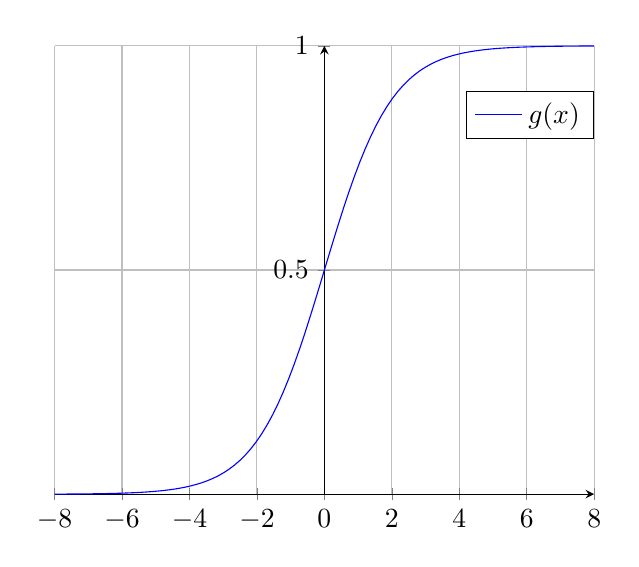
\begin{tikzpicture}[declare function={sigma(\x)=1/(1+exp(-\x));}]
\begin{axis}%
[
    grid=major,     
    xmin=-8,
    xmax=8,
    axis x line=bottom,
    ytick={0,.5,1},
    ymax=1,
    axis y line=middle,
    samples=100,
    domain=-8:8,
    legend style={at={(1,0.9)}}     
]
    \addplot[blue,mark=none]   (x,{sigma(x)});
    \legend{$g(x)$}
\end{axis}
\end{tikzpicture}

Der Wert $h_{\Theta}(x)$ wird als Wahrscheinlichkeit verstanden, dass der Output (y) positive ist für ein gegebener Eingabewert (x) parametrisiert mit $\Theta$.
\linebreak

Formal definiert:
$$h_{\Theta}(x) = P(y=1|x;\Theta)$$
Somit gilt:
$$ P(y=0|x;\Theta) = 1 - P(y=1|x;\Theta)$$



Cost-Function:

$$ J(\Theta) = \frac{1}{m}\sum_{i=1}^{m}Cost(h_{\Theta}(x^{(i)}), y^{(i)}) $$


$$ \text{Cost}(h_{\Theta}(x), y) =
    \begin{cases}
      -\text{log}(h_{\Theta}(x)) & \text{for } y=1\\
      -\text{log}(1 - h_{\Theta}(x)) & \text{for } y=0\\
    \end{cases} $$

Im Gegensatz zur linearen Regression wird bei der logistischen die Cost-Funktion je nach Fall (Wert von y) unterschieden, um eine konvexe Funktion zu generieren.
Graphisch dargestellt sieht die Cost-Function wie folgt aus:

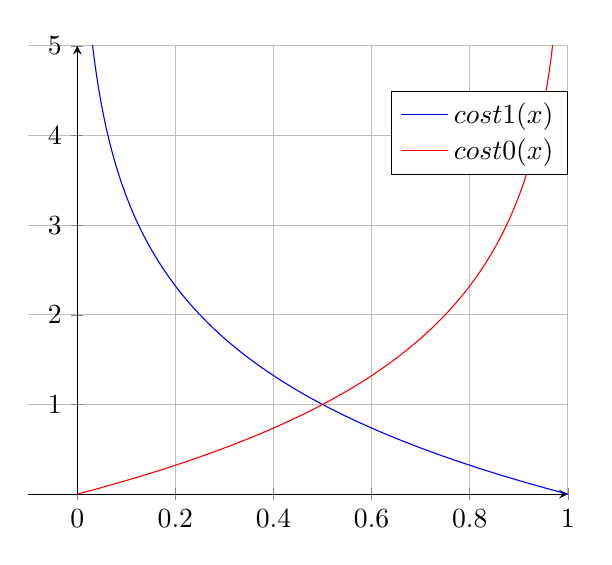
\begin{tikzpicture}[declare function={c1(\x)=-log2(x); c0(\x)=-log2(1-x);}]
\begin{axis}%
[
    grid=major,     
    xmin=-0.1,
    xmax=1,
    axis x line=bottom,
    ytick={0,1,2,3,4,5},
    ymax=5,
    axis y line=middle,
    samples=1000,
    domain=0:1,
    legend style={at={(1,0.9)}}     
]
    \addplot[blue,mark=none]   (x,{c1(x)});
    \addplot[red,]   (x,{c0(x)});
    \legend{$\text{cost1}(x)$, $\text{cost0}(x)$}
\end{axis}
\end{tikzpicture}


\begin{algorithm}
\caption{Calculate $\text{min}_{\Theta} J(\Theta)$}
\begin{algorithmic} 
\REPEAT 
\STATE $ \Theta_{j} := \Theta_{j} - \alpha\sum_{i=1}^{m}(h_{\Theta}(x^{(i)}) - y^{(i)})x_{j}^{(i)} $
\COMMENT{simultaneously update all $\Theta_{j}$}
\UNTIL{$J(\Theta)$ converges}
\end{algorithmic}
\end{algorithm}

Eine Vektor-Implementation dieses Algorithmus sieht so aus:

$$ \Theta := \Theta - \frac{\alpha}{m} X^{T}(g(X\Theta) - \vec{y}) $$

\subsubsection{Regularization}

TODO


% ****************************************
\subsection{Multiclass classification}
\subsubsection{One-vs-all}

Sei $y = {0, 1, ..., n}$ die zu klassifizierenden Klassen. So wird für jede Klasse in y eine logarithmische Regression gebildet. Die entstehende Funktion unterscheidet zwischen der gerade betrachteten Klasse (i) und allen anderen. Daher wird diese Methode auch One-vs-rest genannt.

$$ y \in {0, 1, ..., n} $$

$$ h_{\Theta}^{(0)}(x) = P(y=0|x;\Theta) $$
$$ h_{\Theta}^{(1)}(x) = P(y=1|x;\Theta) $$
$$ \text{...} $$
$$ h_{\Theta}^{(n)}(x) = P(y=n|x;\Theta) $$

$$ \text{prediction} = \text{max}_{i}(h_{\Theta}^{(i)}(x)) $$








\end{flushleft}



